\begin{quote}\emph{This blog is an invited contribution by Dr.~Shengchao Liu; see the \href{http://waveintell.ai/blog/}{Wave Intelligence Lab}.}\end{quote}

\section{Flow Matching: A Physicist's Perspective}

One of the earliest and most influential scientific observations of randomness in nature came from \textbf{Brownian motion}: the irregular movement of pollen particles suspended in water. This phenomenon offered a visible manifestation of microscopic fluctuations and later helped inspire the microscopic theory of gases, in which the macroscopic behaviour of matter is explained through the random motion of an enormous number of particles. Diffusion, a fundamental transport process that appears throughout the physical world, was subsequently studied and formalised by physicists and mathematicians. Their work established the mathematical foundations for describing how particles, energy, or probability distributions spread over time. These ideas later became central to modern transport theory and now provide an important theoretical basis for diffusion-based methods in machine learning, including \textbf{diffusion models} for generative modelling.

Flow matching, one of the state-of-the-art frameworks in generative modelling, also admits a natural interpretation from physics. Its mathematical structure is closely related to transport dynamics in classical mechanics, especially the way probability densities evolve under a prescribed velocity field. This connection makes flow matching not only a powerful machine learning method, but also a conceptually appealing one, since it can be illustrated through well-established physical principles. The dynamics of flow matching are typically defined by the ordinary differential equation

\[
\dot{x}_t = v_t(x_t),
\]

where \(v_t(x)\) is a time-dependent velocity field that transports samples through the data space. Rather than modelling randomness explicitly, this formulation describes deterministic motion along trajectories induced by \(v_t\).

The probability density transported by this flow evolves according to the \textbf{continuity equation}

\[
\partial_t p_t(x) + \nabla \cdot \bigl(p_t(x)\, v_t(x)\bigr) = 0,
\label{keyeq:flow-continuity}
\]

where \(p_t(x)\) denotes the marginal density at time \(t\). This is simply the statement of conservation of probability mass: as particles move under the velocity field \(v_t\), the total probability is preserved, even though the density may locally expand or contract. Following the density along a characteristic trajectory \(x_t\), we obtain

\[
\frac{\mathrm{d}}{\mathrm{d}t} p_t(x_t)
=
-\, p_t(x_t)\, \nabla \cdot v_t(x_t).
\]

This relation shows that the divergence of the velocity field directly controls how the density changes along the flow. When \(\nabla \cdot v_t(x_t) > 0\), the flow locally expands and the density decreases; when \(\nabla \cdot v_t(x_t) < 0\), the flow contracts and the density increases. From this perspective, flow matching can be viewed as learning a transport process that continuously reshapes one probability distribution into another. This transport picture is deeply familiar in physics. Variants of the same continuity structure appear in electrodynamics, fluid mechanics, and quantum mechanics whenever one tracks the evolution of a conserved quantity. A particularly clean example is \textbf{Hamiltonian mechanics}, where the dynamics in phase space are generated by a symplectic vector field. In that case, the flow is volume-preserving, so the divergence vanishes:

\[
\nabla \cdot v_t = 0
\quad \Longrightarrow \quad
\frac{\mathrm{d}}{\mathrm{d}t} p_t(x_t)=0.
\]

Hamilton's equations are

\[
\dot q = \frac{\partial H}{\partial p},
\qquad
\dot p = -\frac{\partial H}{\partial q},
\]

where \(q\) and \(p\) denote position and momentum, respectively. In Hamiltonian mechanics, the motion of a system is represented as a trajectory in \textbf{phase space}, with coordinates \((q, p)\). We then introduce a phase-space density \(\rho(q, p, t)\) describing an ensemble of systems. By conservation of the number of systems in the ensemble, the density satisfies the continuity equation

\[
\frac{\partial}{\partial t}\rho(q, p, t) + \nabla \cdot (\rho v) = 0,
\]

where the phase-space velocity is

\[
v = (\dot q, \dot p).
\]

The divergence of this velocity field is

\[
\nabla \cdot v
= \frac{\partial \dot q}{\partial q} + \frac{\partial \dot p}{\partial p}
= \frac{\partial^2 H}{\partial q\, \partial p} - \frac{\partial^2 H}{\partial p\, \partial q}
= 0.
\]

Thus, Hamiltonian flow preserves phase-space volume, which is the usual statement of \textbf{Liouville's theorem} in classical mechanics. Equivalently, the density remains constant along trajectories:

\[
\frac{\mathrm{d}}{\mathrm{d}t}\rho(q, p, t) = 0.
\]

This gives a useful physical perspective on flow matching. Like Hamiltonian transport, flow matching describes the evolution of a density under a velocity field. The key difference is that flow matching does \textbf{not} require phase-space volume to be preserved. Its learned vector field may expand or contract probability mass locally in order to transform one distribution into another. In this sense, flow matching can be understood as a generalised transport process: it retains the continuity-based structure familiar from physics while relaxing the strict incompressibility that characterises Hamiltonian dynamics.

\begin{quote}
\textbf{Takeaway.} Flow matching is a continuity-driven transport process. Unlike Hamiltonian dynamics, its learned field may compress or expand probability density in order to reshape one distribution into another.
\end{quote}

\section{When Scaling Evolves: From Renormalisation Group to K-Flow}

In traditional flow matching, the introduction of the time parameter \(t\) can feel somewhat artificial. Since the flow is not generally volume-preserving, the notion of time does not arise as naturally from the physical picture discussed above. This motivates a different question: instead of tracking how a system evolves in time, can we describe how it evolves across \textbf{scales}? In condensed matter physics and quantum field theory, this question leads to the \textbf{renormalisation group} (RG). The central idea is that many physical systems exhibit self-similar structure across different length or energy scales, and one therefore seeks a framework that describes how the parameters of an effective theory change as the observation scale varies.

In RG theory, the evolution of a coupling parameter \(g\) with respect to the effective energy scale \(k\) is governed by the \textbf{renormalisation group equation}

\[
\frac{\partial g}{\partial \ln k} = \beta(g),
\]

where \(\beta(g)\) is the beta function, encoding how the effective theory changes with scale. Rather than describing motion in time, this equation describes motion in \textbf{scale space}.

This perspective suggests a natural reinterpretation of generative flow: instead of evolving along an abstract time variable, one may evolve along a physically meaningful scale parameter. A useful intuition comes from the fact that, in many physical systems, energy-like quantities are associated with squared frequency or squared wave number. In quantum mechanics, for example, one often encounters relations of the form

\[
E \propto k^2.
\]

For natural images and other structured signals, analogous scale information can be extracted through \textbf{K-transforms}, such as Fourier or wavelet transforms. If \(\phi_k\) denotes the coefficient at scale \(k\), then it is natural to associate an effective scale-dependent energy with its amplitude:

\[
E_k \propto \|\phi_k\|^2.
\]

This provides a physically motivated way to organise information by scale, rather than by an externally imposed time coordinate. Under this viewpoint, the governing equation of K-Flow can be written as

\[
\frac{\mathrm{d}\Psi_k}{\mathrm{d}k} = v_k(\Psi_k),
\label{keyeq:kflow-dynamics}
\]

where \(\Psi_k\) denotes the observable evolving along the scale parameter \(k\), and \(v_k\) is the corresponding scale-dependent velocity field.

\begin{figure}[htbp]
  \centering
  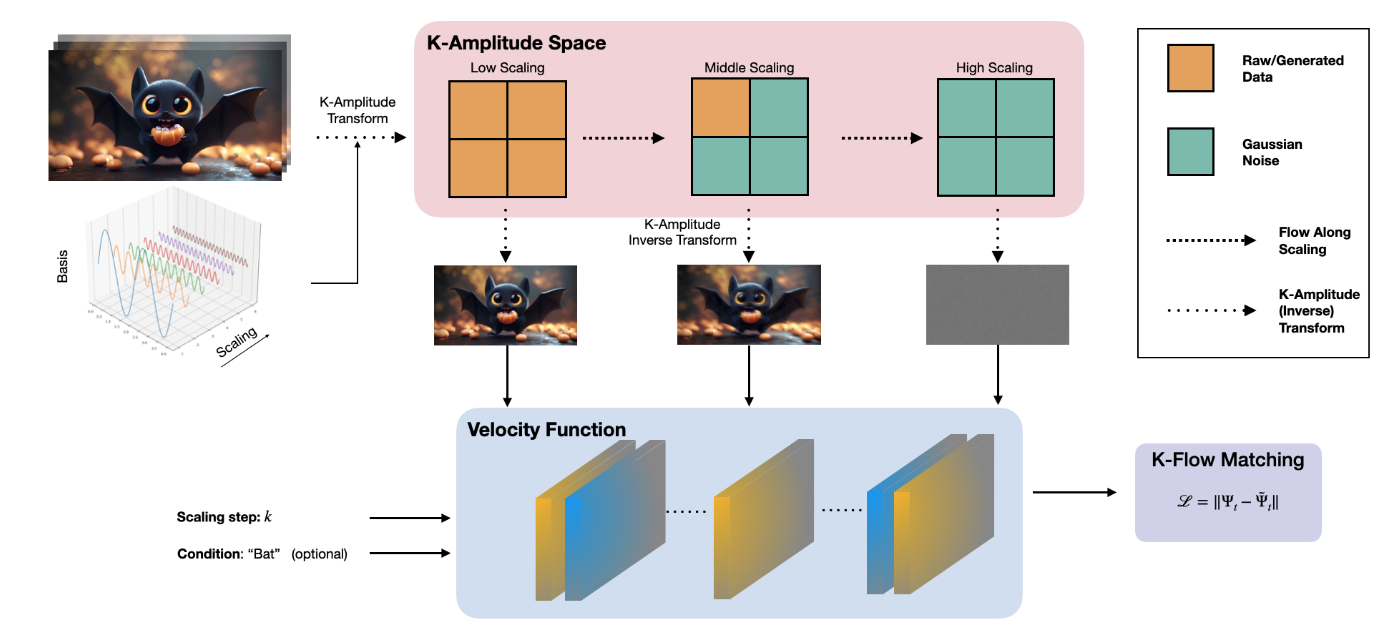
\includegraphics[width=0.94\linewidth]{assets/images/blog/k-flow/k_flow.png}
  \caption{Scale-wise construction used by K-Flow.}
\end{figure}

More concretely, \(\Psi_k\) is constructed by progressively revealing transform coefficients up to scale \(k\), while the remaining components are padded or interpolated with noise:

\[
\Psi_k
=
\mathcal{F}^{-1}
\Big(
\mathbf{1}_{\sqrt{k_x^2+k_y^2+k_z^2}<\lfloor k \rfloor}\,\mathcal{F}\{\phi\}
+
\bigl(1-\mathbf{1}_{\sqrt{k_x^2+k_y^2+k_z^2}\ge \lfloor k \rfloor + 1}\bigr)\epsilon
+
\mathbf{1}_{\sqrt{k_x^2+k_y^2+k_z^2}\in[\lfloor k \rfloor,\lfloor k \rfloor+1)}
\bigl(
\mu(t)\,\mathcal{F}\{\phi\}
+
(1-\mu(t))\,\epsilon
\bigr)
\Big),
\]

where \(\mathbf{1}\) is the indicator function, \(\mathcal{F}\) denotes the chosen K-transform, \(\epsilon\) is noise, and \(t = k-\lfloor k \rfloor\) parameterised the interpolation within a single scale shell. This construction suggests a close analogy with RG:

\[
\frac{\mathrm{d}\Psi_k}{\mathrm{d}k} = v_k(\Psi_k)
\qquad \Longleftrightarrow \qquad
\frac{\partial g}{\partial \ln k} = \beta(g).
\label{keyeq:kflow-rg-analogy}
\]

In both cases, the central object evolves not in physical time, but along a scale parameter that organises the degrees of freedom of the system. From this perspective, K-Flow can be interpreted as a scale-wise transport process, in which information is generated or reconstructed progressively across frequency bands. The analogy is not exact in a strict field-theoretic sense, but it is conceptually useful: RG describes how effective descriptions change with scale, while K-Flow describes how observables are transported across a hierarchy of scales in transform space.

This scale-wise structure also leads to a localised probabilistic interpretation. By the telescoping decomposition of conditional probabilities,

\[
p_t(\cdot)
=
p(k_0)\cdots p_t(\cdot\mid \lfloor k \rfloor,\ldots,k_0)\,
p_{\epsilon}(\lfloor k \rfloor+1)\cdots
p_{\epsilon}(k_{\max}\mid k_{\max}-1,\ldots,k_0),
\]

the marginal distribution at step \(t\) is effectively \textbf{localised} around the current scale shell. In other words, only a restricted band of coefficients is actively being updated, while lower-scale components are already determined and higher-scale components remain noise-dominated.

\begin{figure}[htbp]
  \centering
  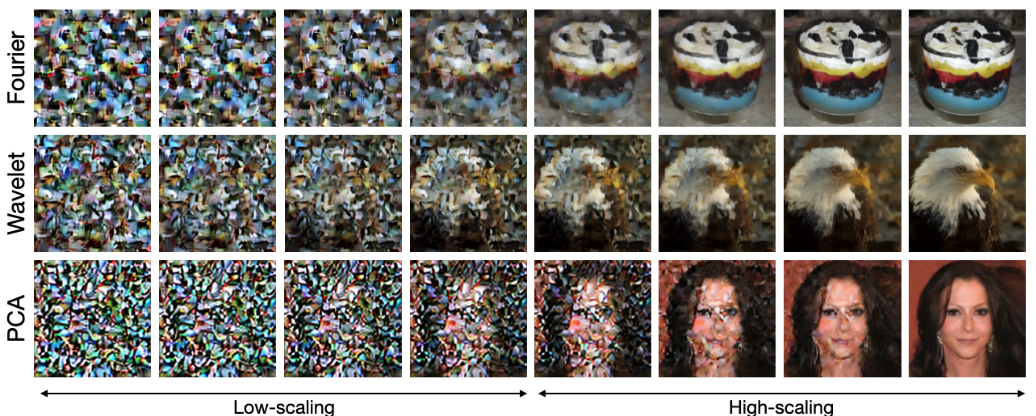
\includegraphics[width=0.94\linewidth]{assets/images/blog/k-flow/scaling.png}
  \caption{Information is revealed progressively across scale shells.}
\end{figure}

This resembles the notion of \textbf{shell localisation} in renormalisation group theory, where one studies how the effective description changes as degrees of freedom are integrated in or out shell by shell. Seen in this way, K-Flow replaces the abstract time variable of conventional flow matching with a more structured and physically interpretable evolution across scales.

\begin{quote}
\textbf{Takeaway.} K-Flow replaces abstract time with transform scale. Information is revealed shell by shell, so each update remains localised around the frequency band currently being generated.
\end{quote}

\section{Performance of K-Flow}

In the K-Flow paper \citep{du2025flow}, we conducted extensive experiments across a variety of datasets, including both \textbf{class-conditional} settings, such as \textbf{ImageNet-256 with a VAE}, and \textbf{unconditional} settings, such as \textbf{CelebA-HQ}.

\begin{figure}[htbp]
  \centering
  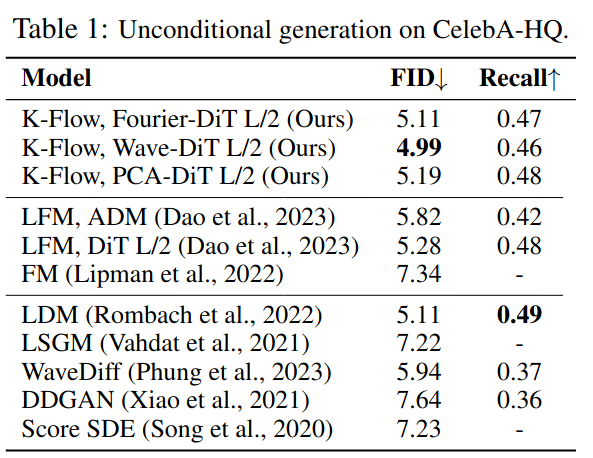
\includegraphics[width=0.47\linewidth]{assets/images/blog/k-flow/res_1.png}
  \hfill
  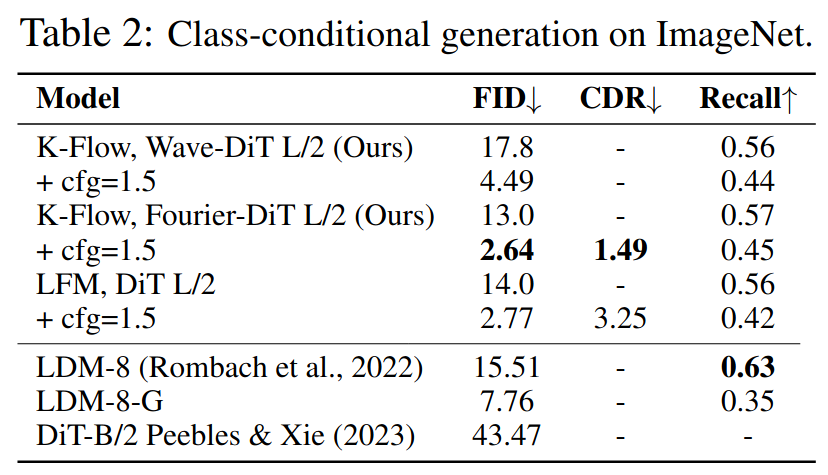
\includegraphics[width=0.47\linewidth]{assets/images/blog/k-flow/res_2.png}
  \caption{Representative K-Flow generation results.}
\end{figure}

Across these benchmarks, K-Flow achieved competitive results, as summarised in \textbf{Tables 1 and 2}. More intriguingly, we observed a striking phenomenon: \textbf{class-conditional labels can be removed at a very early stage of generation without noticeably degrading sample quality}, as illustrated by the samples below.

\begin{figure}[htbp]
  \centering
  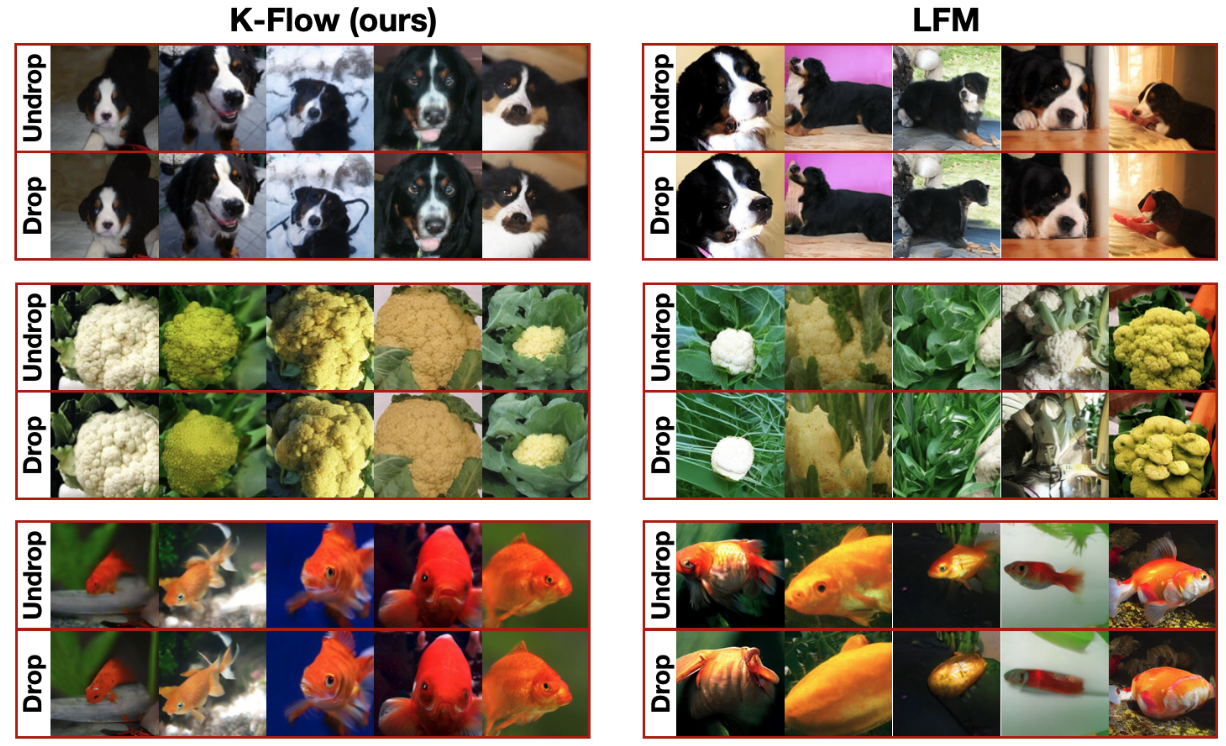
\includegraphics[width=0.78\linewidth]{assets/images/blog/k-flow/cond_drop.png}
  \caption{Conditional-label removal during generation.}
\end{figure}
 This provides strong experimental evidence that our \textbf{energy-driven approach} is learning an internal representation that aligns closely with the \textbf{natural image manifold}, rather than relying solely on label information throughout the entire generation process.

\section{Conclusion and Outlook}

Although our framework is not only theoretically inspiring but also practically effective, the current approach remains significantly constrained by the \textbf{VAE-induced latent space}. This limitation prevents the model from learning an explicit representation directly in pixel space. From both theoretical and applied perspectives, several promising directions remain open:

\begin{enumerate}
\def\labelenumi{\arabic{enumi}.}
\item
  \textbf{Extending K-Flow beyond latent-space generation.}\\
  Can K-Flow be trained directly in pixel space using more efficient architectural designs? More broadly, can the K-Flow formulation be adapted to \textbf{parameter-efficient fine-tuning (PEFT)} settings, allowing it to improve the efficiency of existing pre-trained models?
\item
  \textbf{Applying K-Flow to scientific generation tasks.}\\
  Can the K-Flow framework be used in scientific domains where there exists a genuinely interpretable energy functional? Such settings may offer an opportunity to test the theoretical foundations of K-Flow more directly and rigorously.
\end{enumerate}

We believe these questions open up exciting opportunities for future work.

Please consider citing our paper if you found this work interesting or useful!

